\section{Resultados}

% LES COPIO LO QUE TENGO ANOTADO EN EL CUADERNO:
% Dar parametros de contexto (info sobre LANs usadas y resultados observados, no conclusiones).
\subsection{Implementaci\'on de un cliente ARP}

De todos los casos mencionados en la secci\'on \ref{sec:metodos_1}, el \'unico en que se recibi\'o una respuesta con la direcci\'on MAC solicitada es en el caso (1), es decir, al pedir direcciones MAC de nodos presentes dentro de la red local. En todos los otros casos el mensaje ARP no recibi\'o respuesta alguna.\\

A trav\'es del uso de \emph{Wireshark} pudimos observar con un poco m\'as de detalle qu\'e ocurri\'o en cada una de estas situaciones.\\

El caso (1) funcion\'o como se esperaba: al paquete \emph{who-has} (enviado de manera broadcast) le sigue un paquete \emph{is-at}, con el host cuya MAC se quiere conocer como origen, y dirigido \'unicamente a la m\'aquina que pregunt\'o.\\

Si se pregunta por una IP que no existe, pero que tiene una m\'ascara correspondiente con la red local (por ejemplo, 192.168.0.2), no se observa ning\'un tipo de respuesta. Sin embargo, si se pregunta por un direcci\'on cuya m\'ascara no se corresponde con la red (casos 4, 6, 7, 8\footnote{En el caso de una direcc\'on inv\'alida, la direcci\'on enviada se traduce a una direcci\'on IP correcta (en este caso se envi\'o el paquete pregunt\'ando por la direcci\'on 7.91.205.21).} y 9) se observa un intercambio de mensajes ligeramente diferente. En vez de enviar un paquete ARP de manera broadcast, la m\'aquina pregunta primero qui\'en tiene la direcci\'on (en nuestro caso) 192.168.0.1 (direcci\'on del router). Al recibir la respuesta \emph{is-at} con la MAC correspondiente, pregunta espec\'ificamente al router qui\'en tiene la direcci\'on buscada. Es decir, pareciera ser que antes de enviar mensajes ARP, autom\'aticamente se calcula si dicha IP se encuentra dentro de la red local. Si no se encuentra, se ejecuta el intercambio mencionado, enviando el pedido por la IP buscada directamente al router (del cual no se recibe respuesta, al menos en los casos probados).\\

%Por \'ultimo, si se pregunta por la IP de la misma m\'aquina, observamos a trav\'es del wireshark el siguiente comportamiento. El pedido mencionado genera en la red un paquete ARP cuya IP fuente no es la misma m\'aquina, sino el router (en nuestro caso se observa el siguiente mensaje: \texttt{``Who has 192.168.0.3? Tell 192.168.0.1''}. A este pedido le segu\'ia una respuesta del tipo \emph{is-at} con la informaci\'on correspondiente. De este intercambio no se obtiene sin embargo una respuesta final a la m\'aquina que origin\'o el paquete ARP con su misma IP. 
% LO SAQUE PORQUE NO FUNCIONA ASI LA SEGUNDA VEZ QUE LO CORRO



\subsection{Captura de tr\'afico}

% poner resultados de entropia de cada red
Como mencionamos, se escucharon durante varias horas distintos tipos de redes. A partir de los datos obtenidos calculamos la entrop\'ia de la manera explicada en la secci\'on anterior. Los resultados obtenidos fueron los siguientes:\\

\begin{center}
  \begin{tabular}{l l}
    Captura de c\'atedra: big\_arp.pcap & 7.057\\
    Captura de c\'atedra: small\_arp.pcap & 6.227\\
    Red hogare\~na & 6.749\\
    Red de oficina & 7.428 \\
  \end{tabular}
\end{center}



$\\$
A continuaci\'on se muestran los gr\'aficos generados a partir de los datos obtenidos en esta secci\'on.

\subsubsection{Grafos}
\begin{figure}[h!]
  \centering
    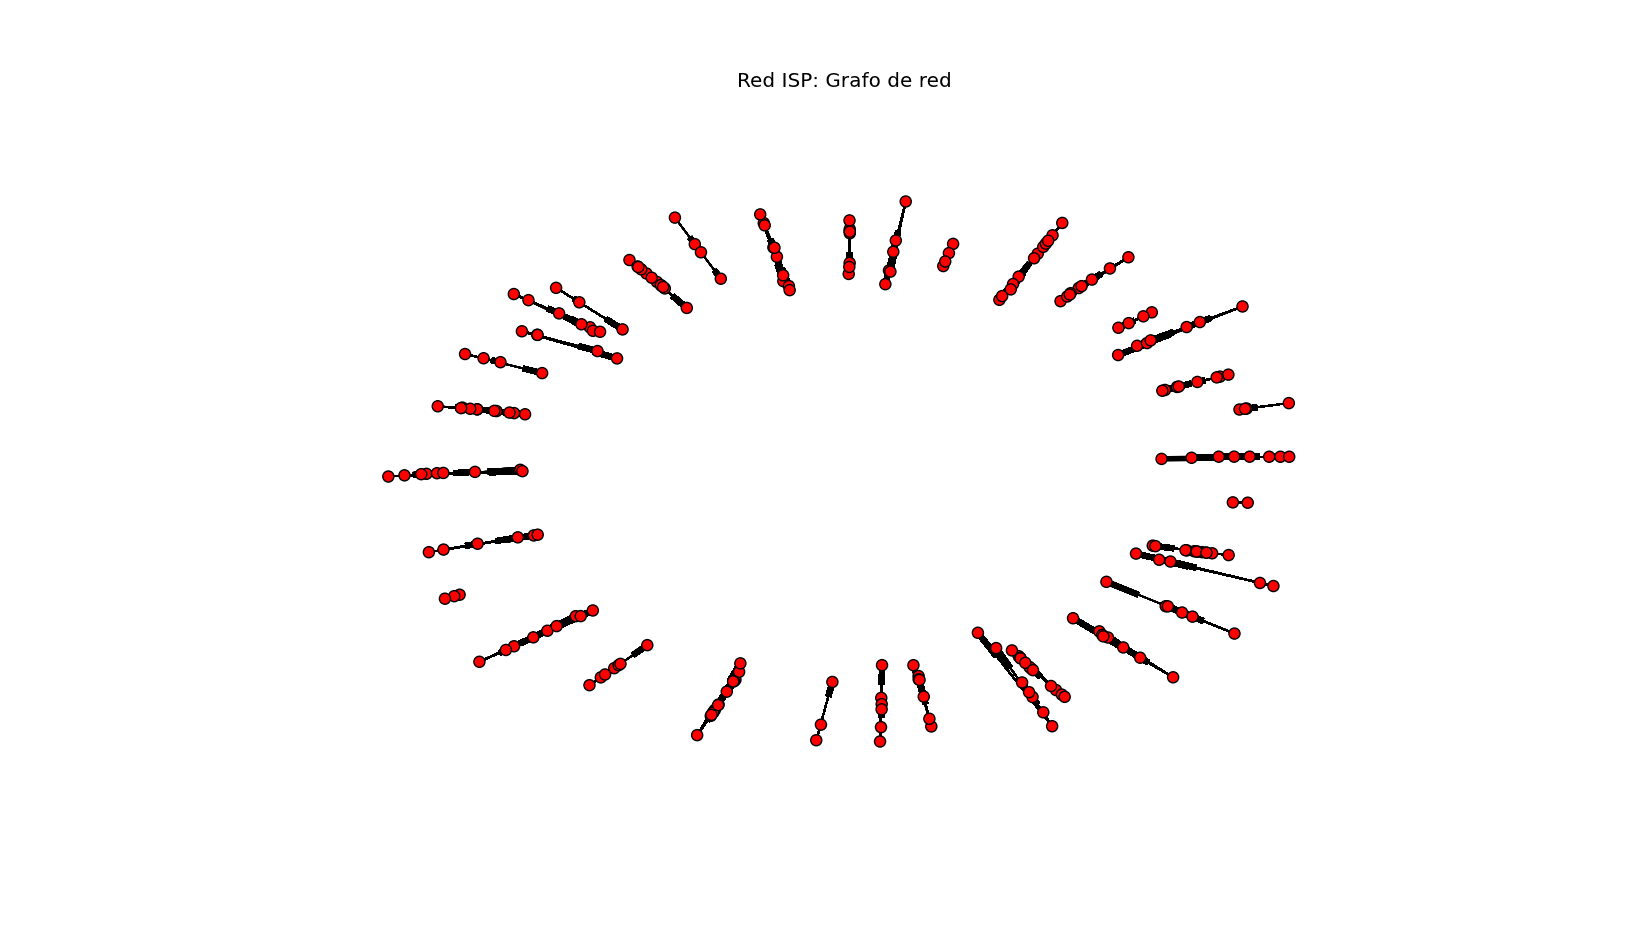
\includegraphics[width=0.8\textwidth]{graficos/grafoCasa.png}
    \caption{Grafo de IPs - Red Hogare\~na}
    \label{fig:grafo1}
\end{figure}

Lo más notable de la figura \ref{fig:grafo1}, como se verá en contraste con los siguientes, es que presenta numerosas componentes conexas pequeñas. Atribuimos esta disposición a que, dado que corresponde con una red de ISP, la interacción, en principio, no se da entre cualqueir par de nodos por igual, ya que obedece a motivos \emph{personales} de los usuarios. De todas formas, la inconexión da la idea de que no existe un nodo centralizador a través del cual se canalice el tráfico (típicamente un router), con lo cual el funcionamiento de la red sería imposible. Por lo tanto, suponemos que, por razones del proveedor, esa información no se transmite via ARP (puede utilizar otros protocolos), o se controla el tráfico de paquetes ARP con destinos sensibles para la red.

\begin{figure}[h!]
  \centering
    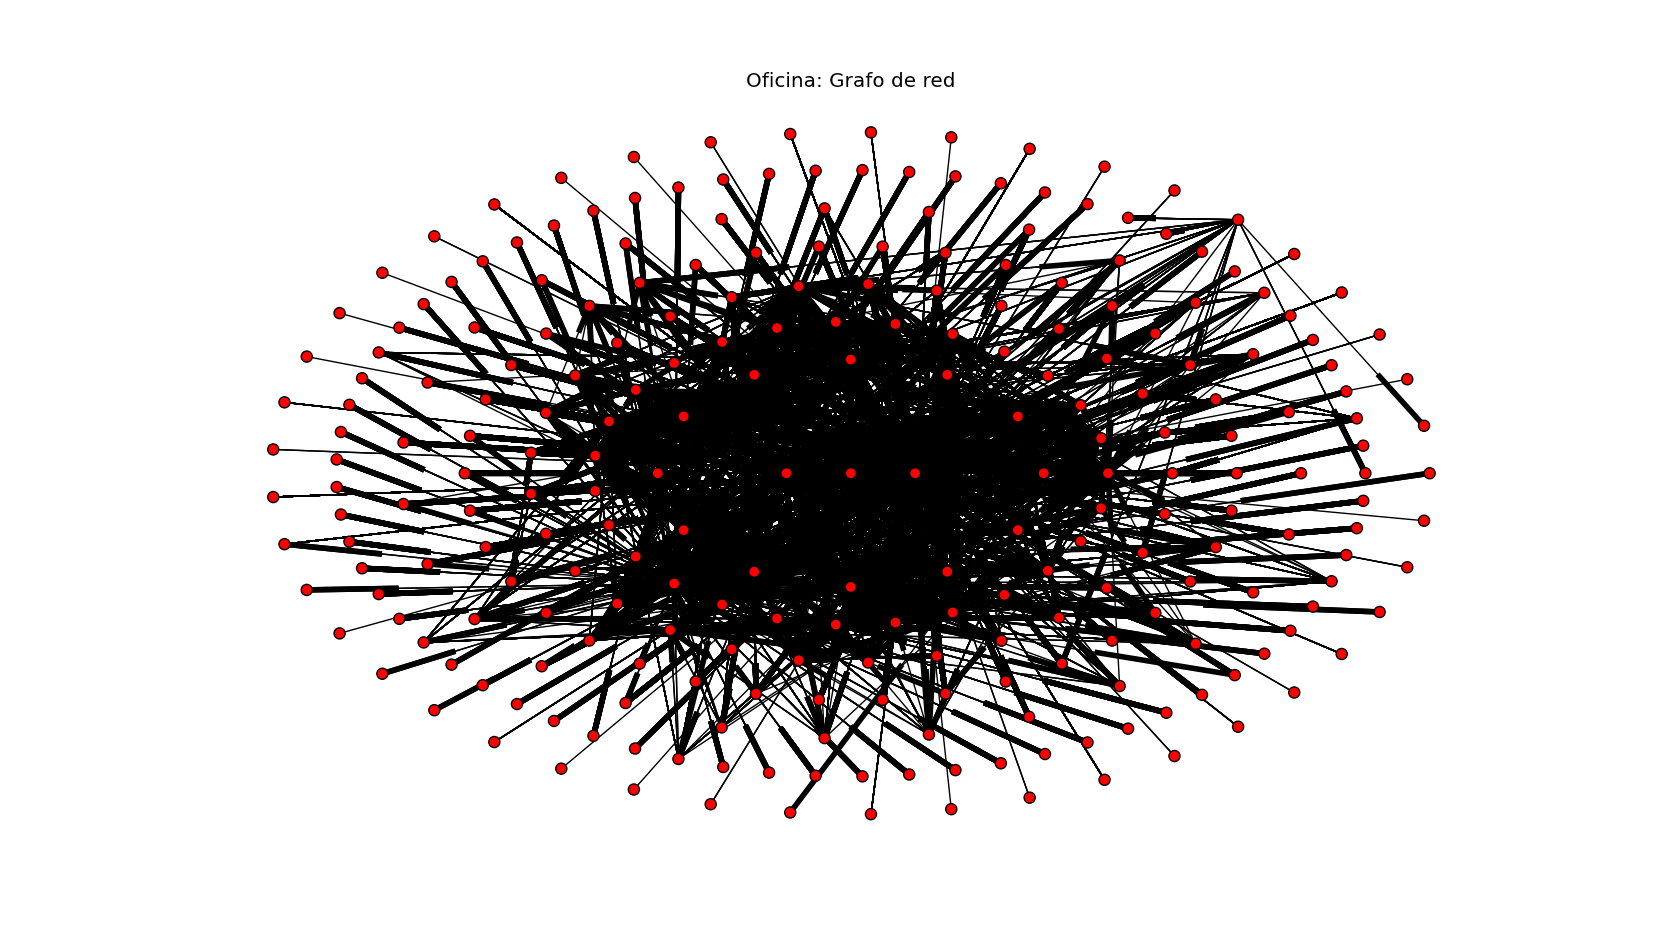
\includegraphics[width=0.8\textwidth]{graficos/grafoOficina.png}
    \caption{Grafo de IPs - Red de Oficina}
    \label{fig:grafo2}
\end{figure}

En el caso de la figura \ref{fig:grafo2}, observamos todo lo contrario al caso anterior. Recordemos que los nodos ubicados más al centro corresponden con las direcciones más solicitadas, típicamente routers/gateways. El alto grado de conexión entre  los nodos centrales refleja la intensa actividad que ocurre entre los hosts en una red privada (ej: clientes de chat). También se observan nodos en el círculo exterior que, no sólo realizan pocas consultas ARP, sino que también nunca le son respondidas. Estos pueden ser dispositivos que se conectaron por poco tiempo y para realizar una tarea espefícica, o direcciones inválidas que no fueron consideradas por el resto de la red para recibir datos.

\begin{figure}[h!]
  \centering
    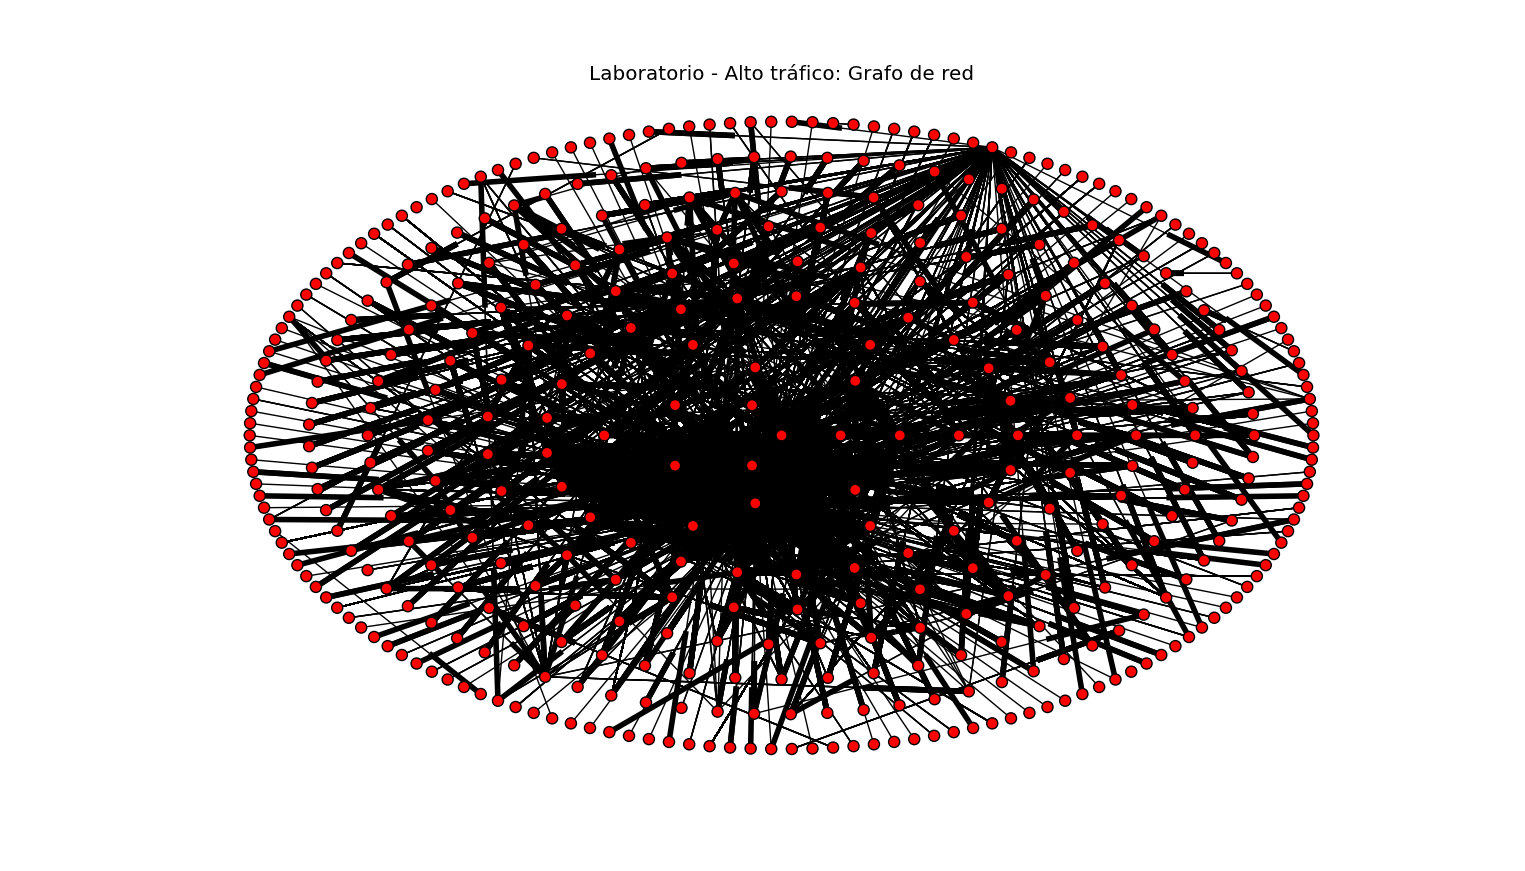
\includegraphics[width=0.8\textwidth]{graficos/grafoLaboBig.png}
    \caption{Grafo de IPs - big\_arp.pcap}
    \label{fig:grafo3}
\end{figure}

Para el grafo de la figura \ref{fig:grafo3}, se observa algo similar que en la figura \ref{fig:grafo2}. Pocos nodos con un alto nivel de solicitudes, y una disposición numerosa a su alrededor. Cabe el mismo análisis que en el caso anterior, destacando también la presencia de un nodo del círculo exterior que realiza numerosos pedidos, pero que no le son respondidos en la misma medida. Nuevamente, atribuimos este hecho a la presencia de direcciones anómalas (por ejemplo, $0.0.0.0$).

\begin{figure}[h!]
  \centering
    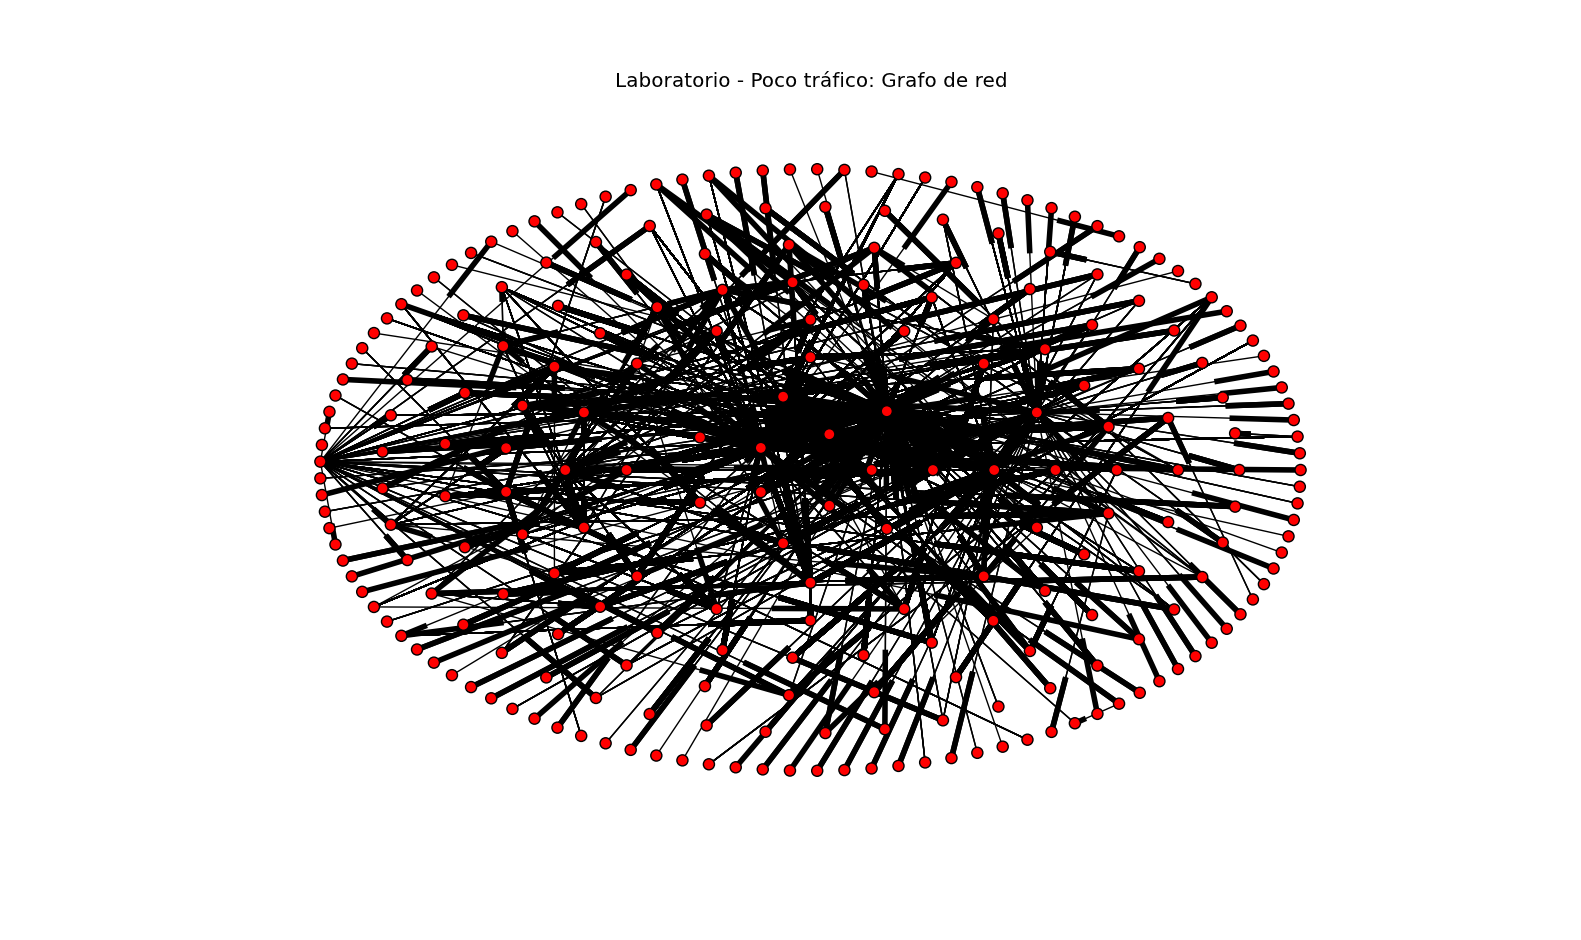
\includegraphics[width=0.8\textwidth]{graficos/grafoLaboSmall.png}
    \caption{Grafo de IPs - small\_arp.pcap}
    \label{fig:grafo4}
\end{figure}

Por último, en la figura \ref{fig:grafo4} vemos un esquema similar a los anteriores, pero dado a que el nivel de tráfico es menor, se aprecian mejor los enlaces. Igualmente existen las direcciones anómalas y los nodos distinguidos en el centro, pero se puede apreciar mejor el intercambio entre los nodos menos distinguidos de la red.

\subsubsection{Histogramas}

\begin{figure}[H]
        \begin{subfigure}[H]{0.5\textwidth}
                \centering
                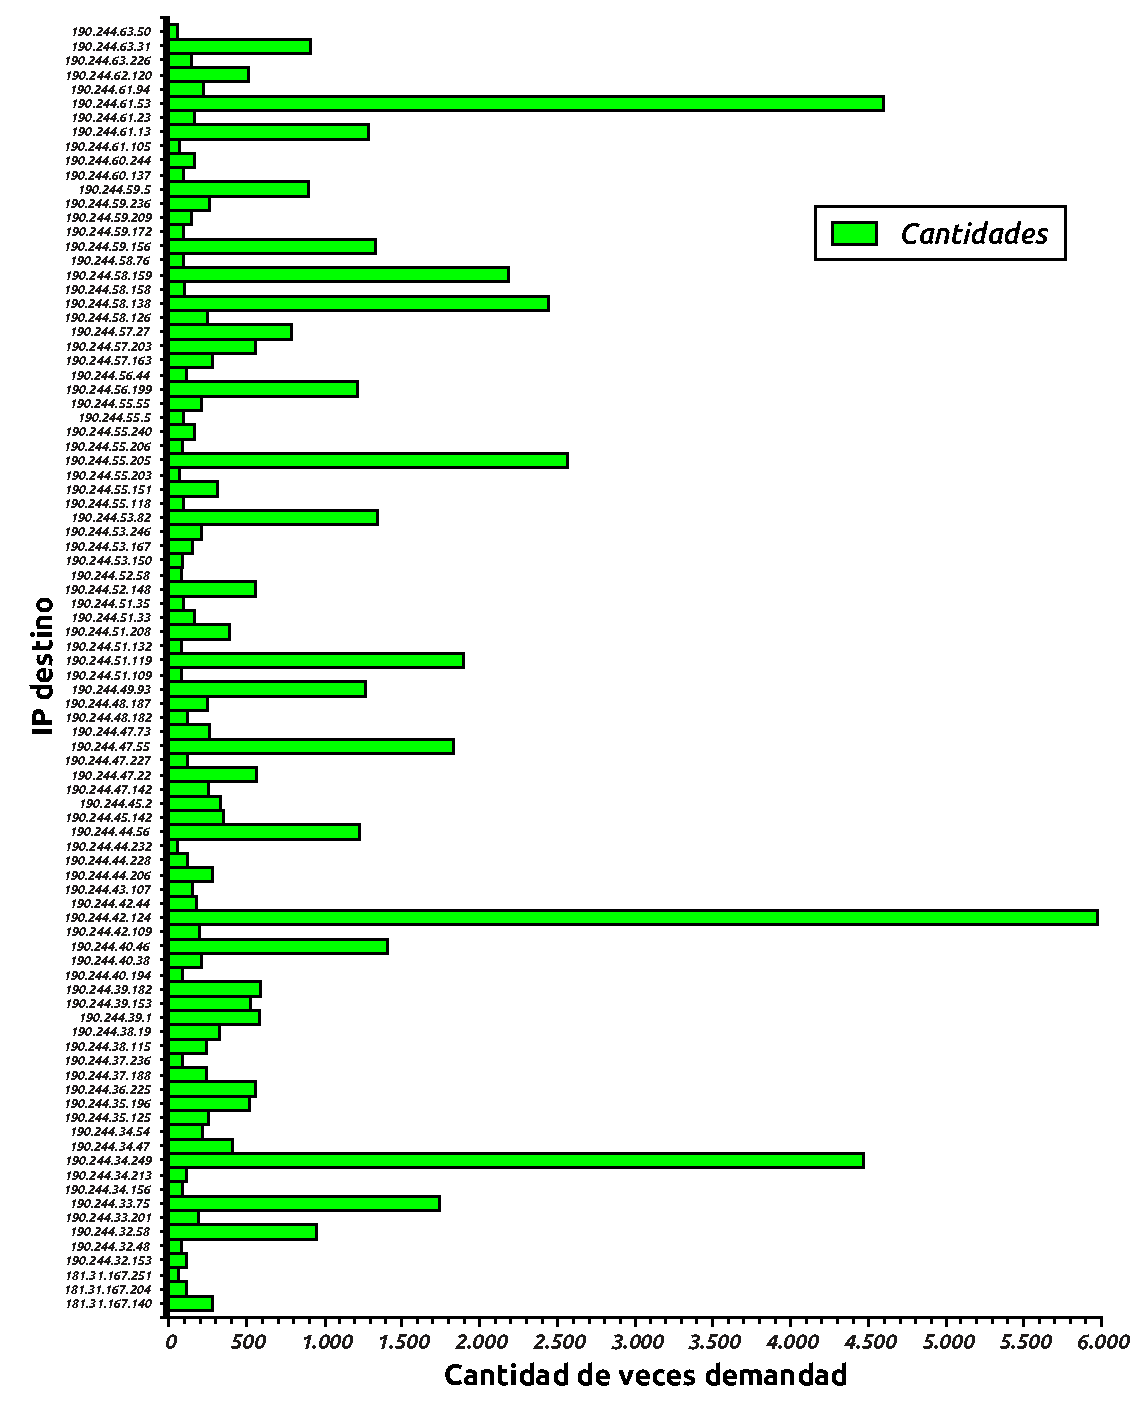
\includegraphics[width=1\textwidth]{graficos/cantidadConsultasCasaJulian.pdf}
                \caption{Cantidad de demandas a cada IP - Red ISP}
                \label{fig:hist1}
        \end{subfigure}
        \begin{subfigure}[H]{0.5\textwidth}
                \centering
                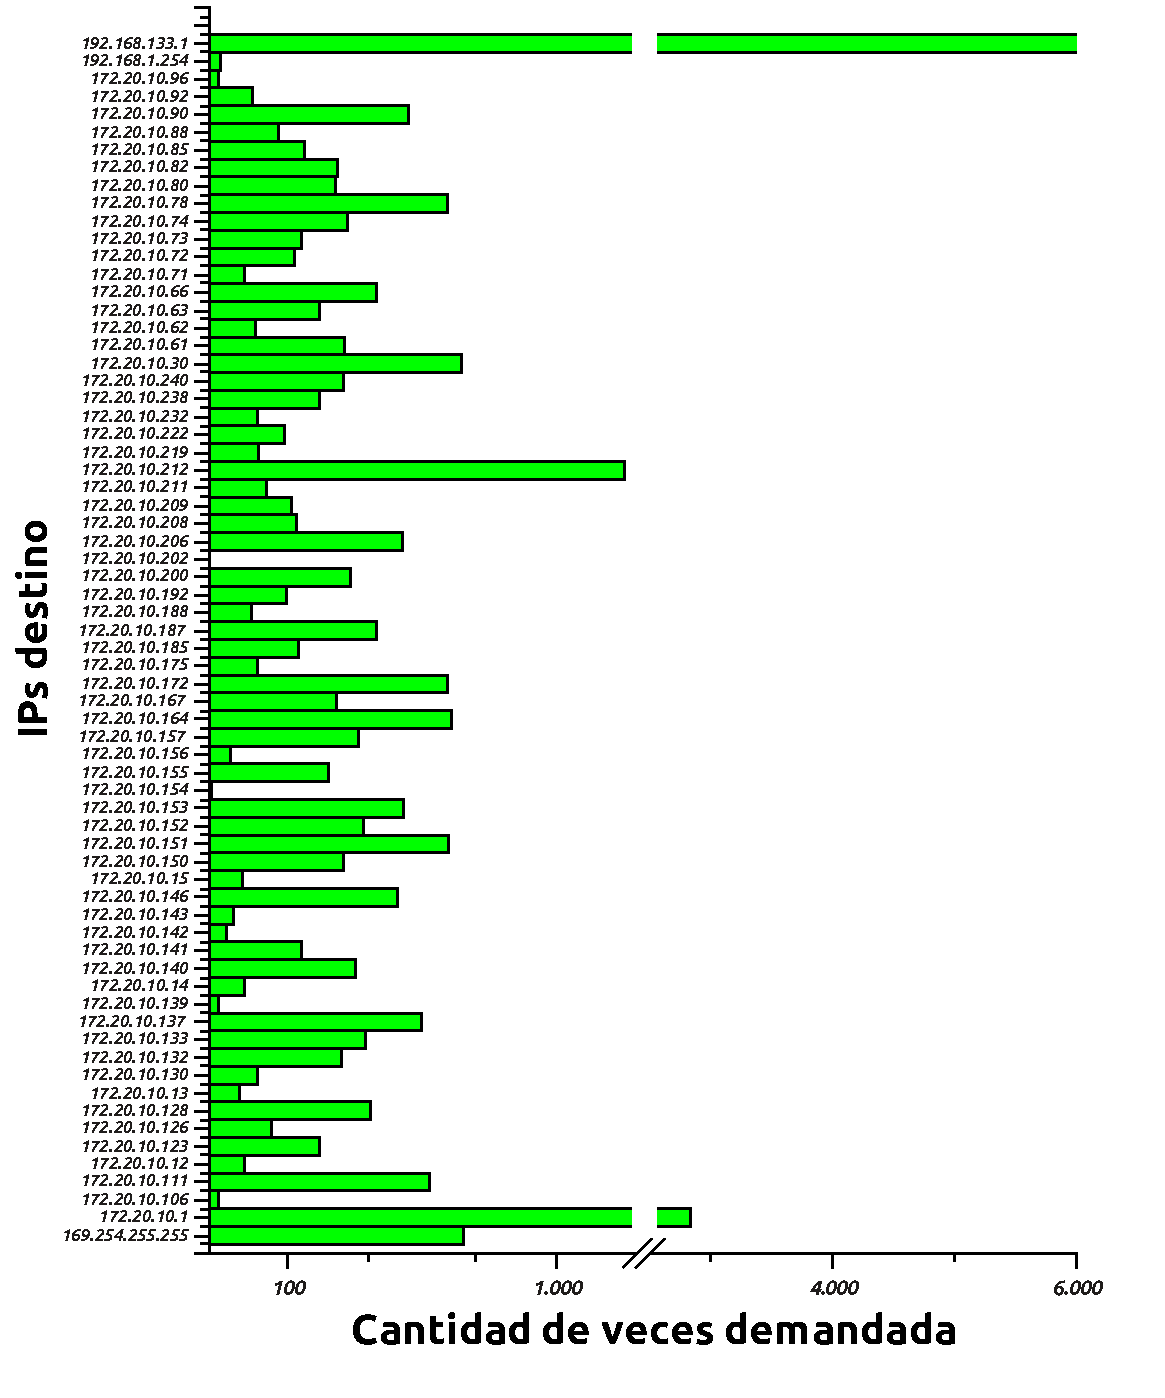
\includegraphics[width=1\textwidth]{graficos/cantidadConsultasOficina.pdf}
                \caption{Cantidad de demandas a cada IP - Oficina}
                \label{fig:hist2}
        \end{subfigure}
\end{figure}

\begin{figure}[H]
        \begin{subfigure}[H]{0.5\textwidth}
                \centering
                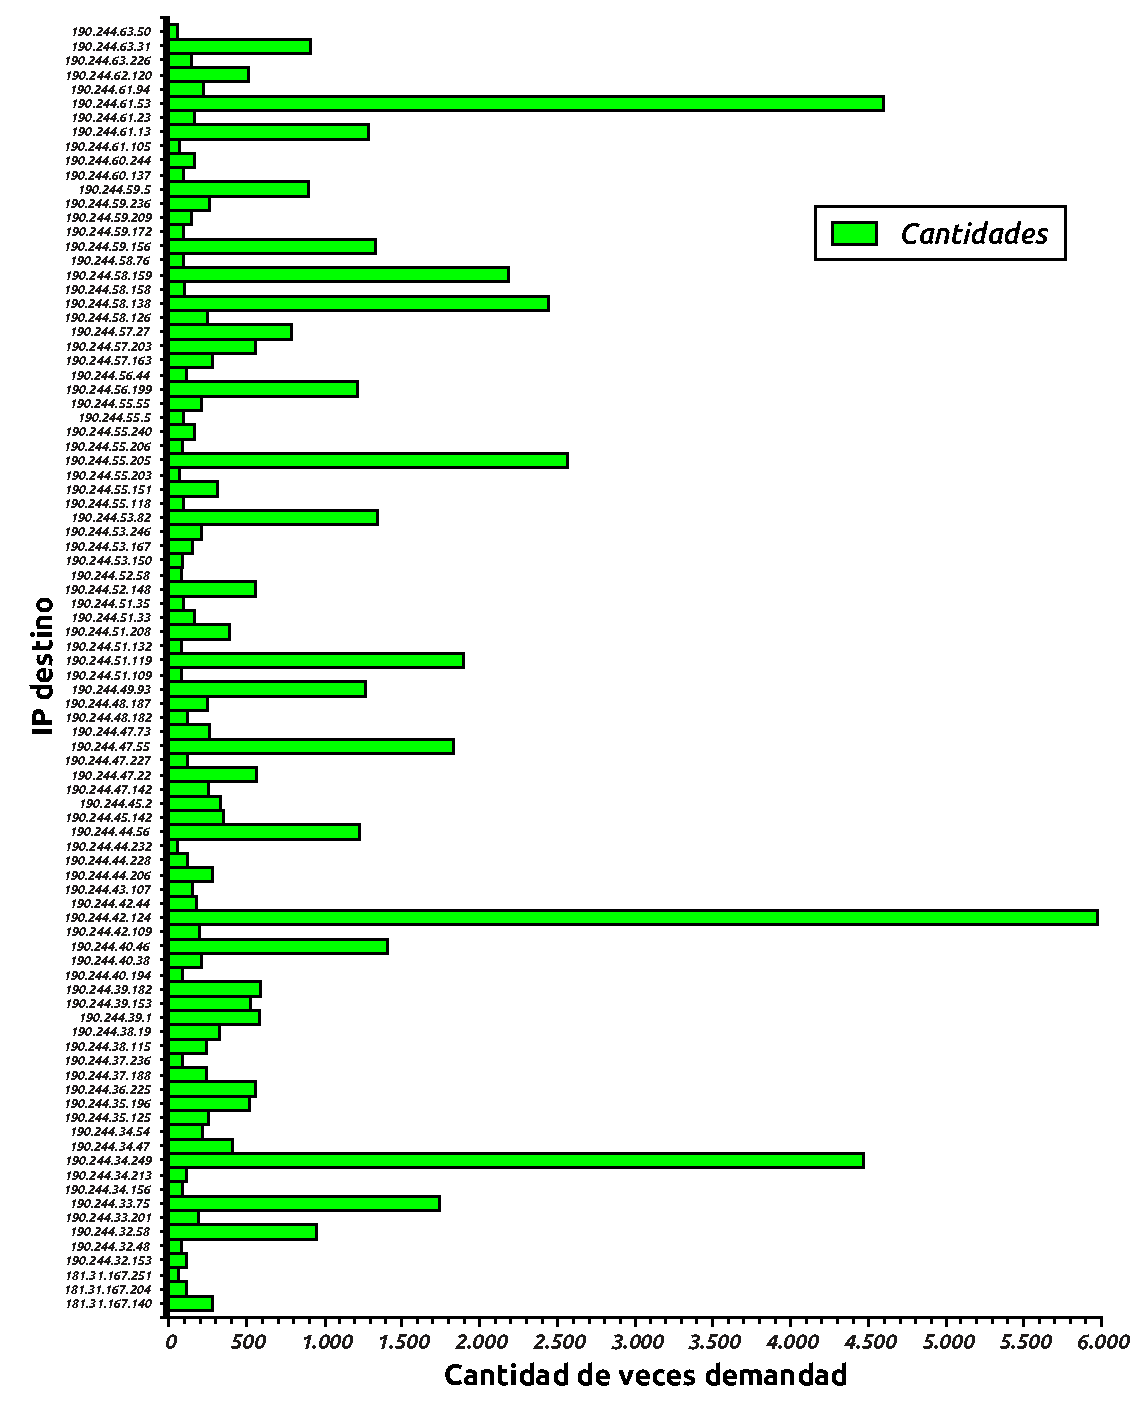
\includegraphics[width=1\textwidth]{graficos/cantidadConsultasCasaJulian.pdf}
                \caption{Cantidad de demandas a cada IP - big\_arp.pcap *** FALTA!!}
                \label{fig:hist3}
        \end{subfigure}
        \begin{subfigure}[H]{0.5\textwidth}
                \centering
                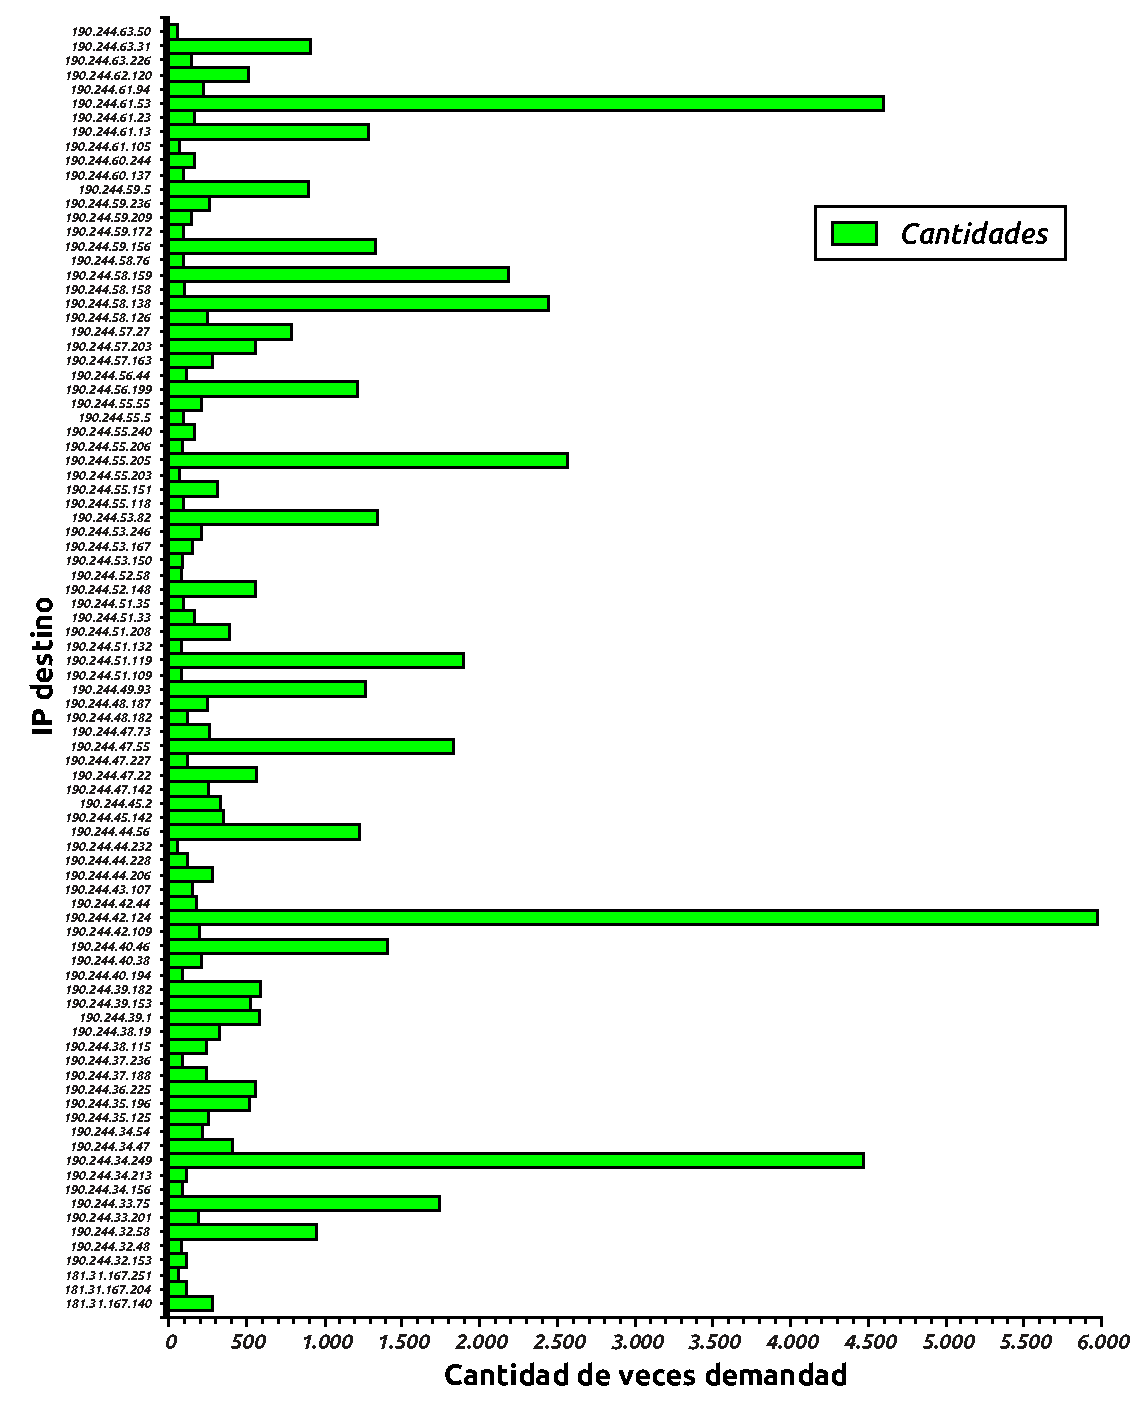
\includegraphics[width=1\textwidth]{graficos/cantidadConsultasCasaJulian.pdf}
                \caption{Cantidad de demandas a cada IP - small\_arp.pcap *** FALTA}
                \label{fig:hist4}
        \end{subfigure}
\end{figure}

\begin{figure}[H]
	\centering
	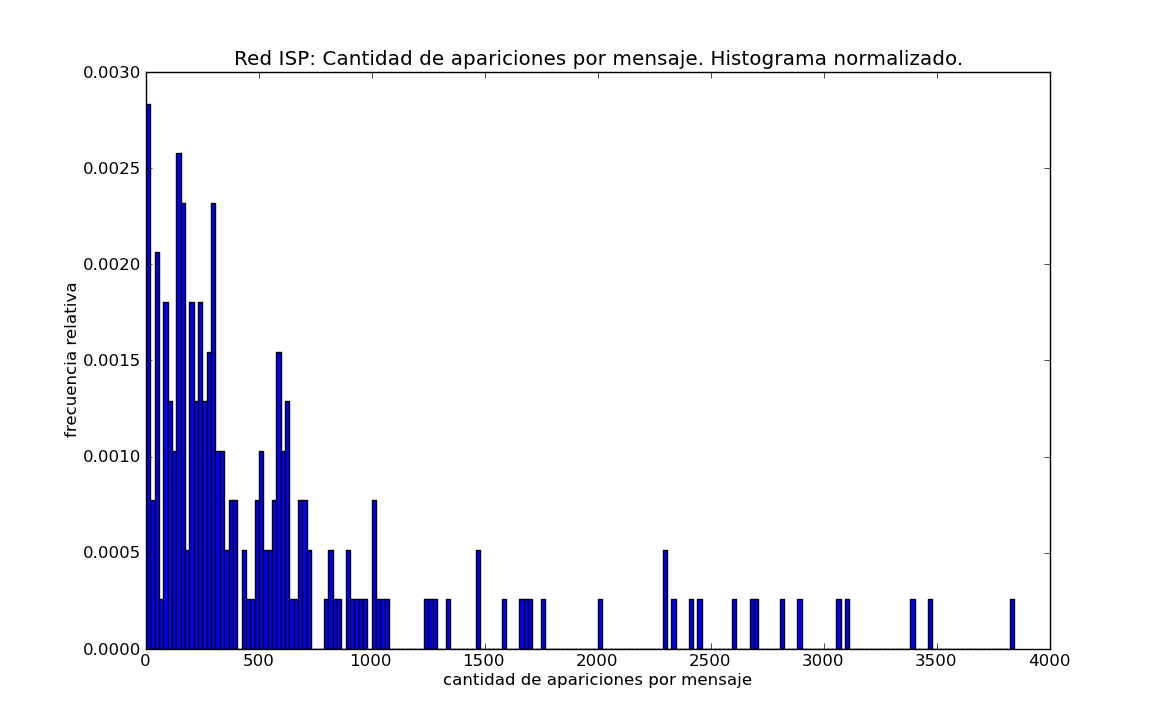
\includegraphics[width=0.8\textwidth]{graficos/hist_casa.png}
	\caption{Cantidad de apariciones de cada mensaje ARP - Red ISP}
	\label{fig:hist5}
\end{figure}

\begin{figure}[H]
	\centering
	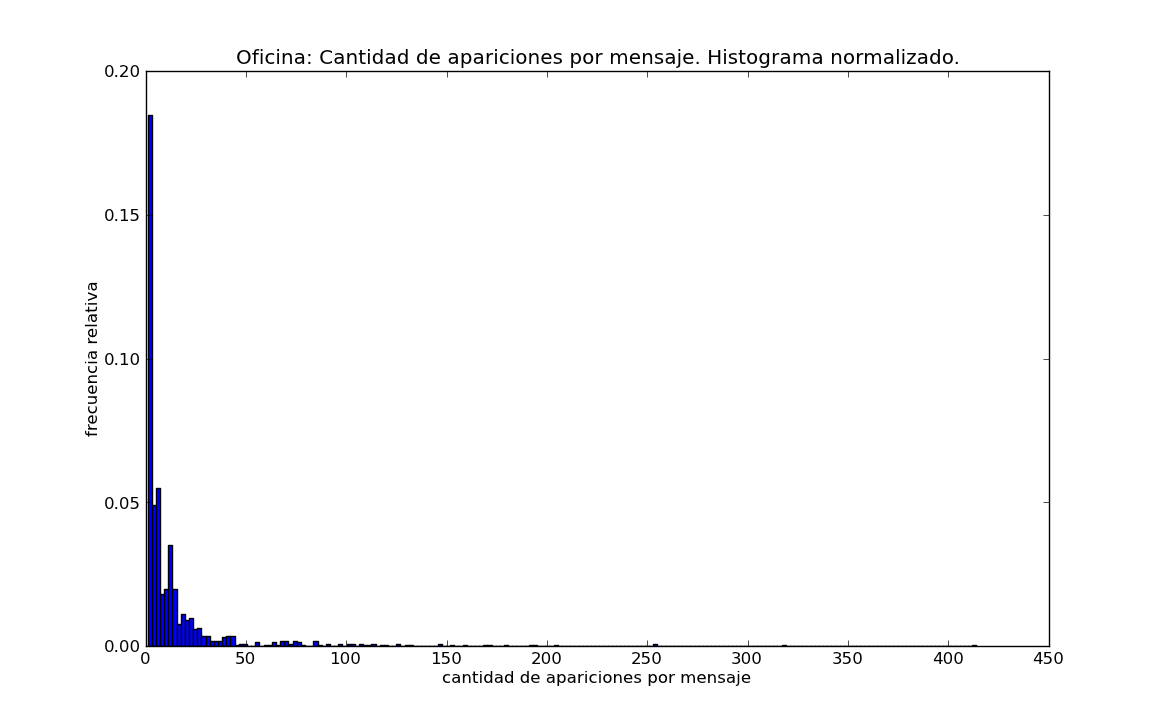
\includegraphics[width=0.8\textwidth]{graficos/hist_oficina.png}
	\caption{Cantidad de apariciones de cada mensaje ARP - Oficina}
	\label{fig:hist6}
\end{figure}

\subsubsection{Informaci\'on de los nodos}

\begin{figure}[H]
        \begin{subfigure}[H]{0.5\textwidth}
                \centering
                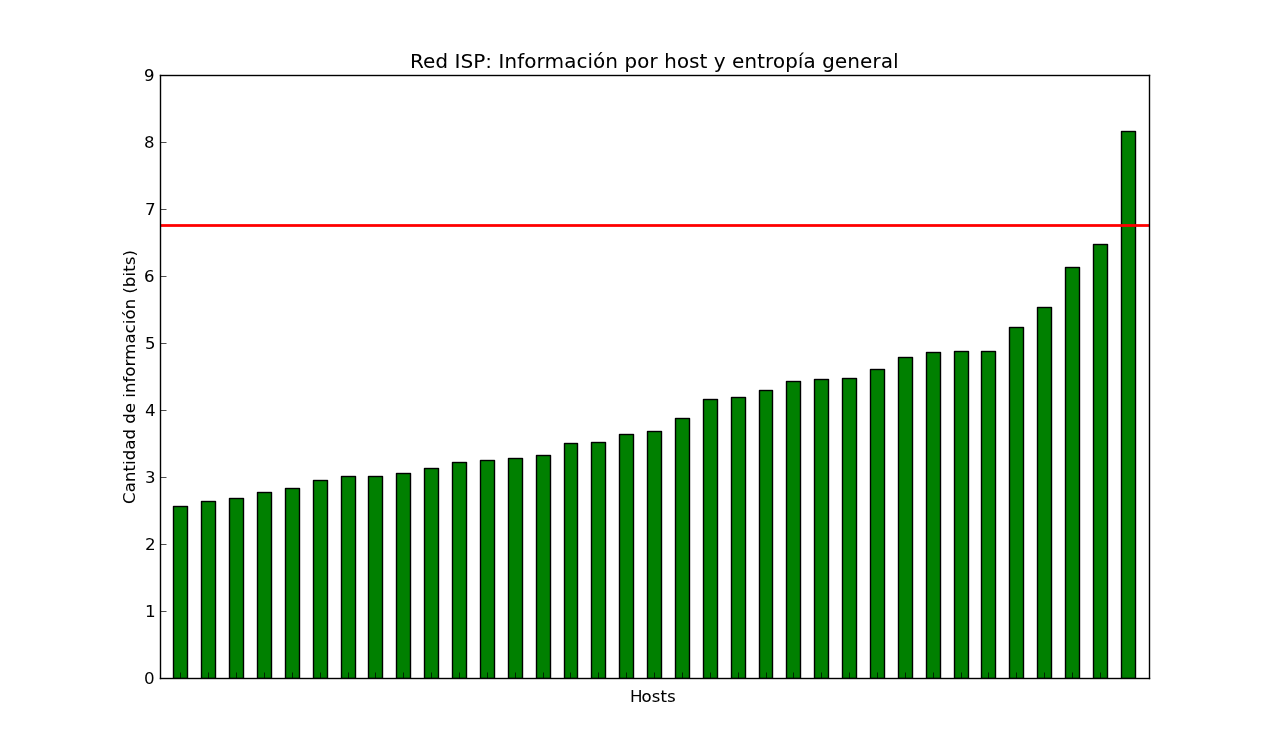
\includegraphics[width=1\textwidth]{graficos/infoHost_casa.png}
                \caption{Cantidad de informaci\'on seg\'un host - Red ISP}
                \label{fig:info1}
        \end{subfigure}
        \begin{subfigure}[H]{0.5\textwidth}
                \centering
                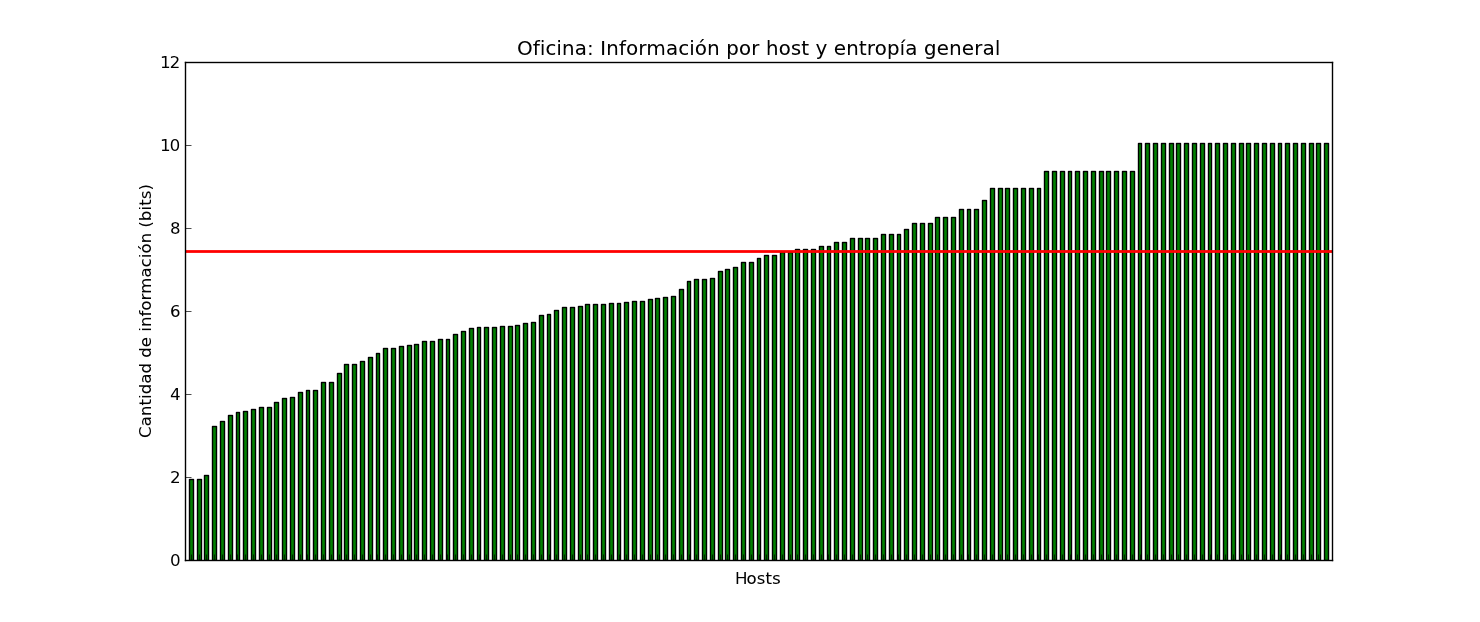
\includegraphics[width=1\textwidth]{graficos/infoHost_oficina.png}
                \caption{Cantidad de informaci\'on seg\'un host - Oficina}
                \label{fig:info2}
        \end{subfigure}
\end{figure}

\begin{figure}[H]
        \begin{subfigure}[H]{0.5\textwidth}
                \centering
                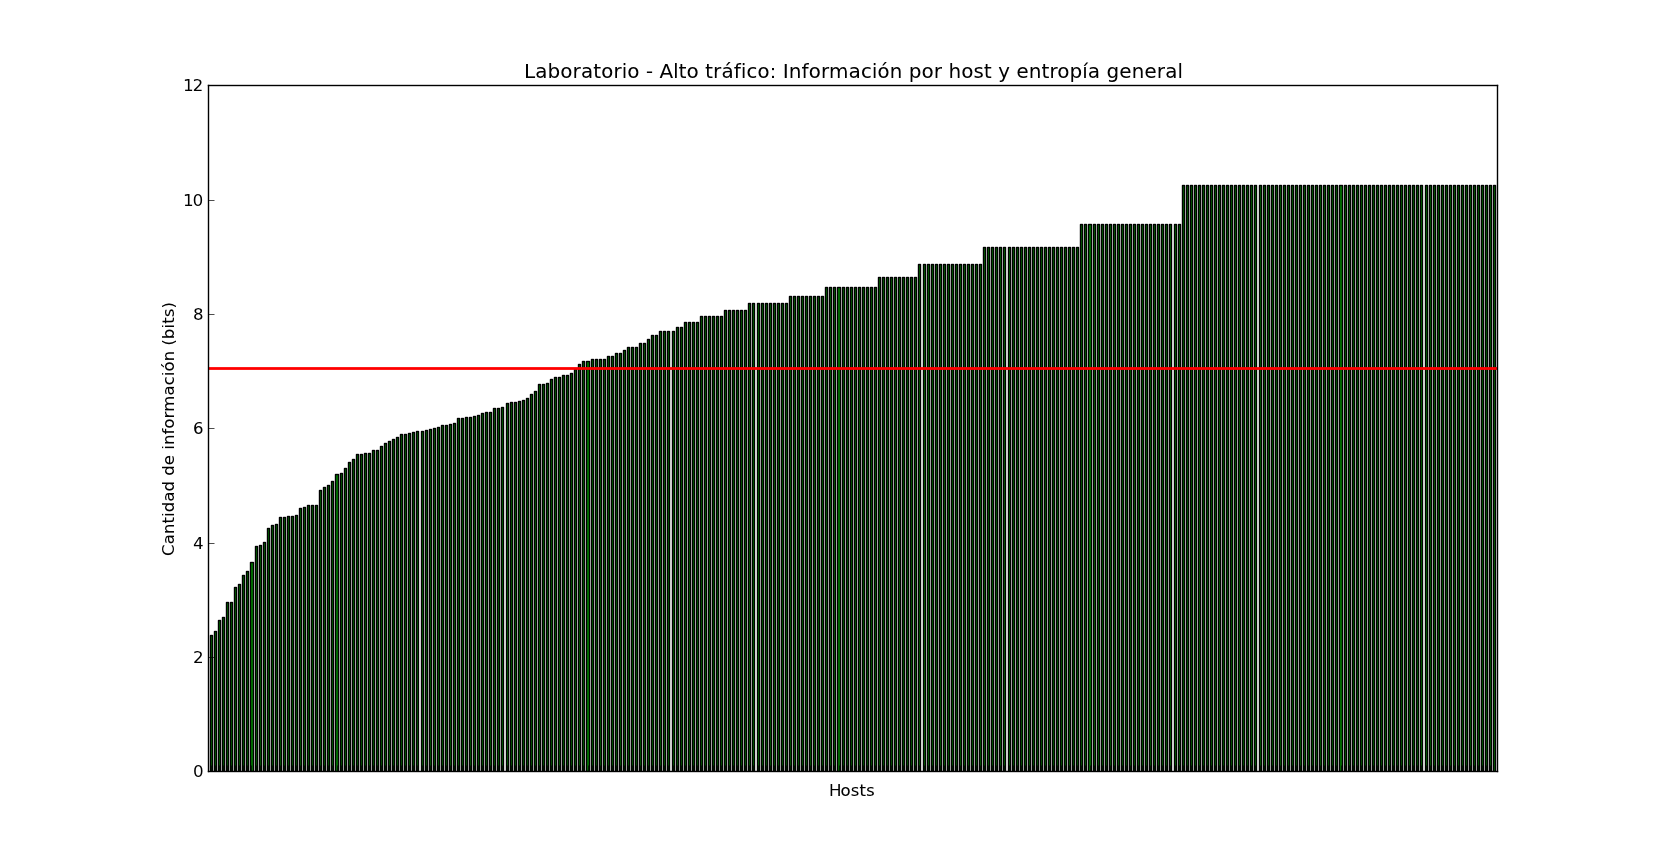
\includegraphics[width=1\textwidth]{graficos/infoHost_laboBig.png}
                \caption{Cantidad de informaci\'on seg\'un host - big\_arp.pcap}
                \label{fig:info3}
        \end{subfigure}
        \begin{subfigure}[H]{0.5\textwidth}
                \centering
                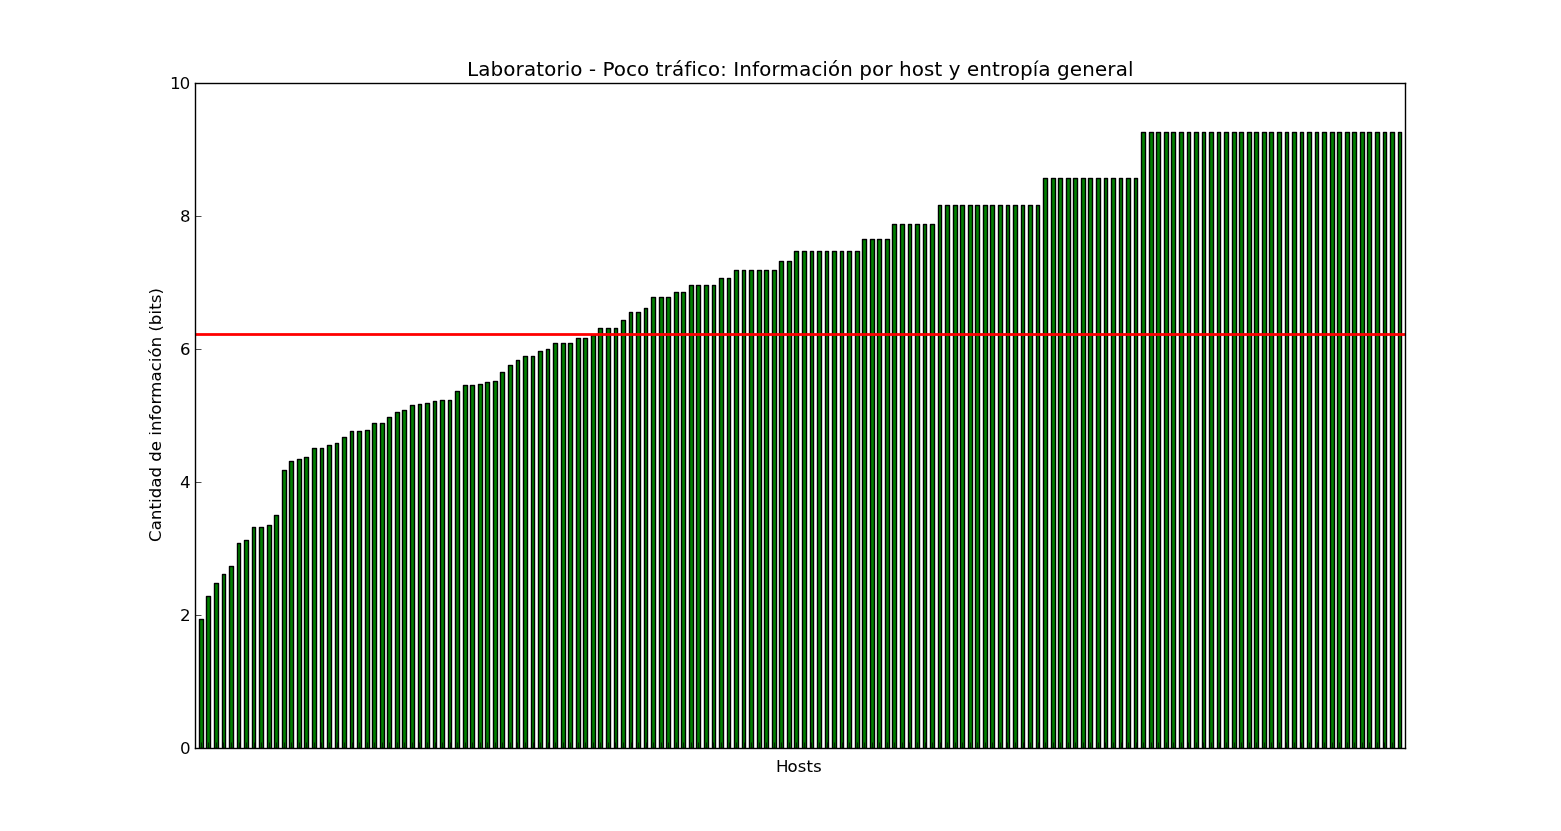
\includegraphics[width=1\textwidth]{graficos/infoHost_laboSmall.png}
                \caption{Cantidad de informaci\'on seg\'un host - small\_arp.pcap}
                \label{fig:info4}
        \end{subfigure}
\end{figure}


\subsubsection{Mediciones en funci\'on del tiempo}

\begin{figure}[H]
        \begin{subfigure}[H]{0.5\textwidth}
                \centering
                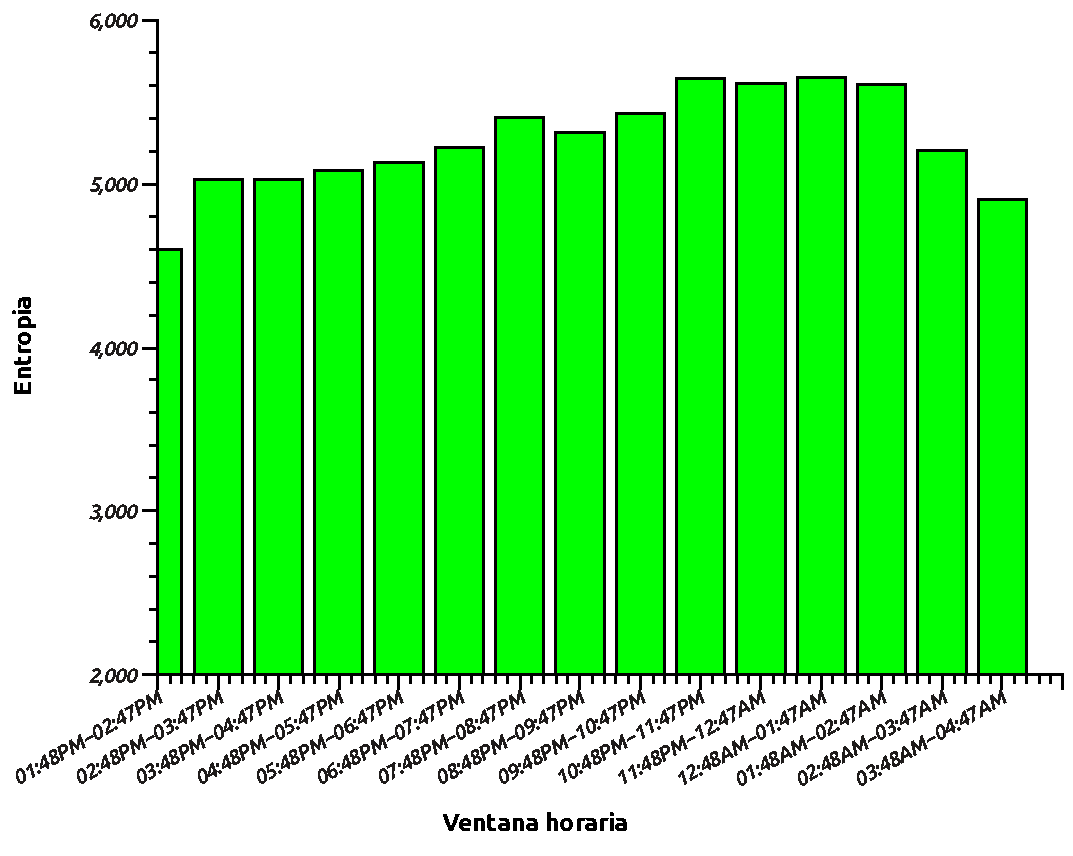
\includegraphics[width=1\textwidth]{graficos/entropiaXHora.pdf}
                \caption{Entrop\'ia en funci\'on de la franja horaria - Red ISP  *** FALTA!}
                \label{fig:paquetes1}
        \end{subfigure}
        \begin{subfigure}[H]{0.5\textwidth}
                \centering
                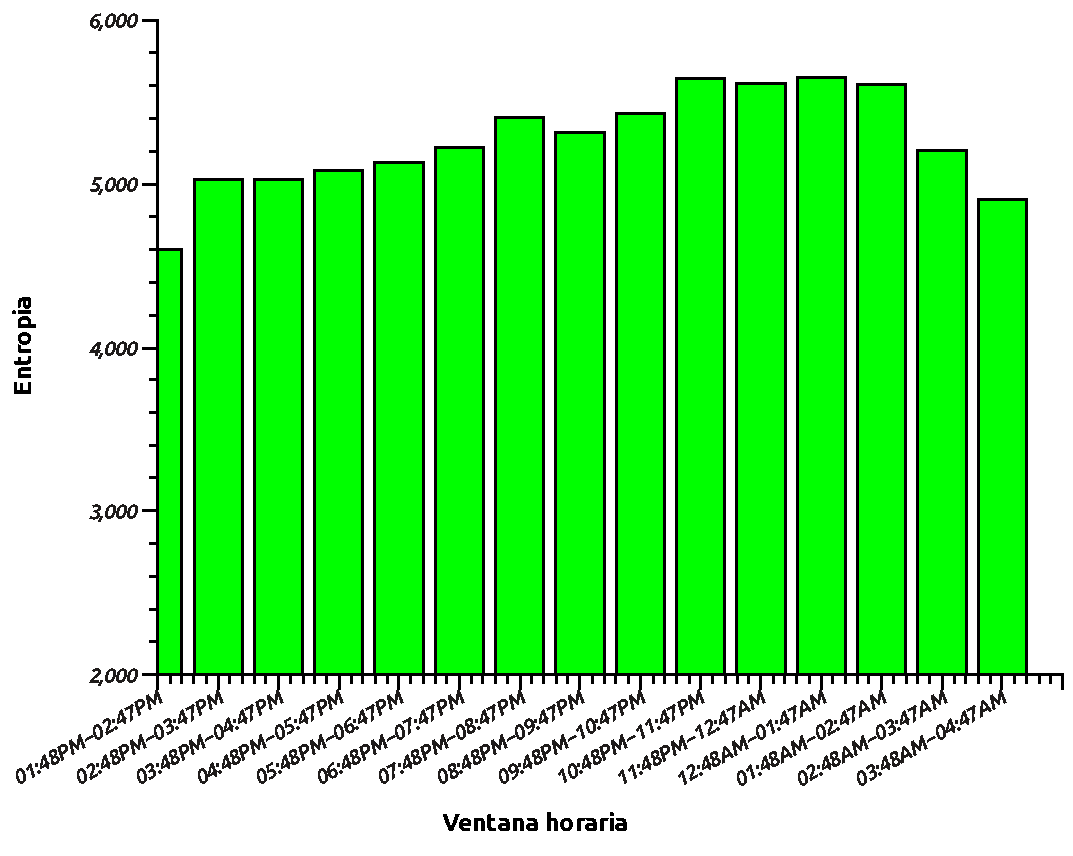
\includegraphics[width=1\textwidth]{graficos/entropiaXHora.pdf}
                \caption{Entrop\'ia en funci\'on de la franja horaria - Oficina}
                \label{fig:paquetes2}
        \end{subfigure}
\end{figure}

\begin{figure}[H]
        \begin{subfigure}[H]{0.5\textwidth}
                \centering
                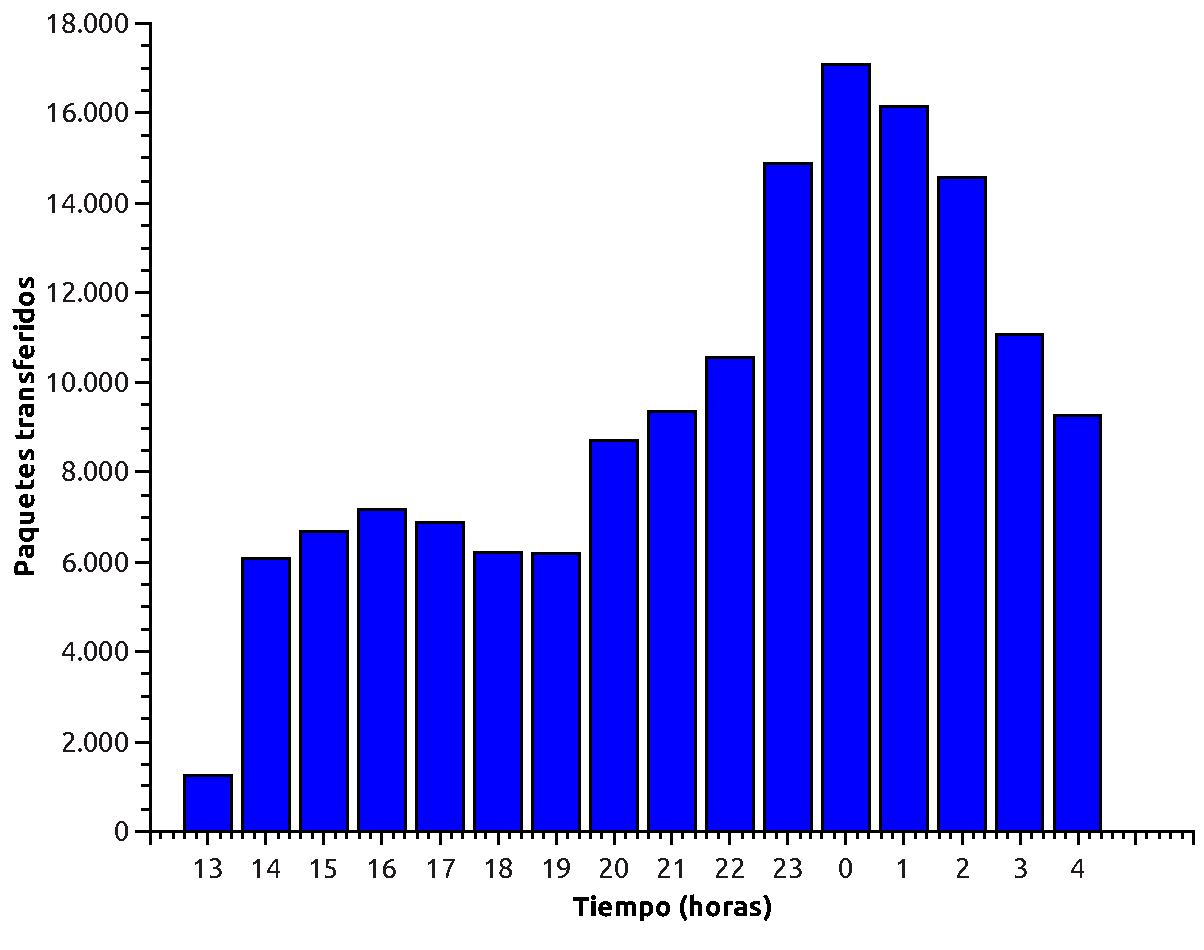
\includegraphics[width=1\textwidth]{graficos/paquetesVsTiempoCasa.pdf}
                \caption{Cantidad de paquetes enviados en funci\'on de la franja horaria - Red ISP}
                \label{fig:paquetes1}
        \end{subfigure}
        \begin{subfigure}[H]{0.5\textwidth}
                \centering
                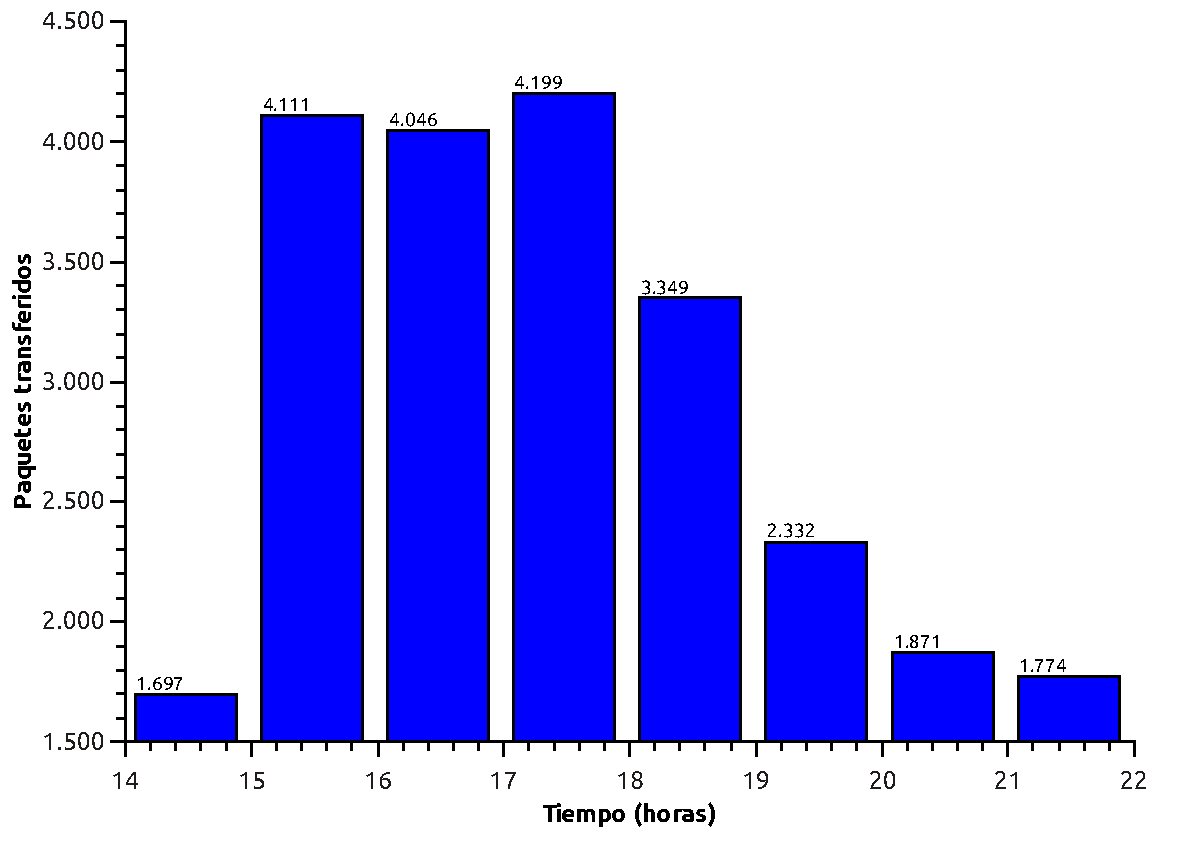
\includegraphics[width=1\textwidth]{graficos/paquetesVsTiempoOficina.pdf}
                \caption{Cantidad de paquetes enviados en funci\'on de la franja horaria - Oficina}
                \label{fig:paquetes2}
        \end{subfigure}
\end{figure}
